\documentclass{article}

\usepackage[utf8]{inputenc}
\usepackage{xeCJK}
\usepackage{kotex}
\usepackage{minted}
\usepackage{mdframed}
\usepackage{ntheorem}
\usepackage{fontspec}
\usepackage{color}
\usepackage{graphicx}
\usepackage[a4paper, top=15mm, bottom=15mm, left=20mm, right=20mm]{geometry}
\setmainfont{NanumGothic}
\setmonofont{D2Coding}

\definecolor{codeblockbackground}{RGB}{245, 245, 245}
\definecolor{codeblockborder}{RGB}{200, 200, 200}

\theoremstyle{nonumberplain}
\newmintedfile[javacode]{java}{
  linenos=true,
  breaklines,
  framesep=2mm,
  bgcolor=codeblockbackground
}
\newminted[console]{text}{
  breaklines,
  framesep=2mm,
  bgcolor=codeblockbackground
}
\newmdtheoremenv[%
  backgroundcolor=codeblockbackground,
  linecolor=codeblockborder,
  outerlinewidth=3
]{code}{}

\graphicspath{ {./tex/} }

\title{자바프로그래밍및실습 과제 5}
\author{214823 컴퓨터정보통신공학과 박종현}
\date{June 2022}

\begin{document}

\maketitle
\pagebreak


코드 주석은 Javadoc 코드 문서화 스펙을 참조하여 작성함.

참조: https://docs.oracle.com/en/java/javase/17/docs/specs/javadoc/doc-comment-spec.html


\section{과제 1}

\subsection{과제 1.1}
\subsubsection{소스 코드}
\javacode{java/Prob1/Prob1.1/Prob1.1.java}
\subsubsection{실행 예제}
\makebox{
  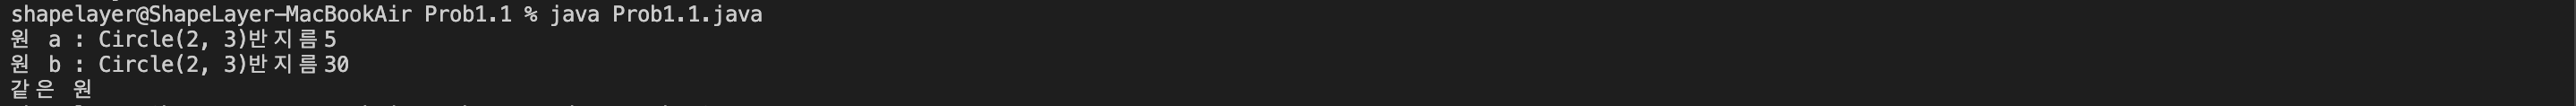
\includegraphics[width=\linewidth]{Prob1.1}
}

\subsection{과제 1.2}
\subsubsection{소스 코드}
프로그램 진입점
/java/Prob1/Prob1.2/main.java
\javacode{java/Prob1/Prob1.2/main.java}
/java/Prob1/Prob1.2/etc/Calc.java
\javacode{java/Prob1/Prob1.2/etc/Calc.java}
\subsubsection{실행 예제}
\makebox{
  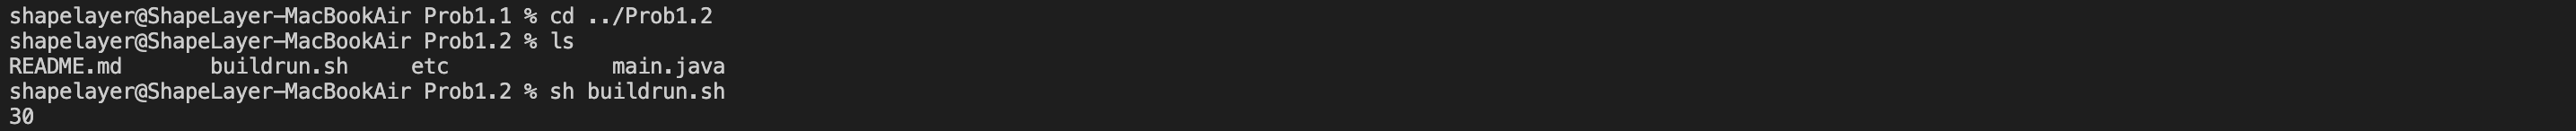
\includegraphics[width=\linewidth]{Prob1.2}
}

\subsection{과제 1.3}
\subsubsection{소스 코드}
프로그램 진입점
/java/Prob1/Prob1.3/app/GraphicEditor.java
\javacode{java/Prob1/Prob1.3/app/GraphicEditor.java}
/java/Prob1/Prob1.3/base/Shape.java
\javacode{java/Prob1/Prob1.3/base/Shape.java}
/java/Prob1/Prob1.3/derived/Circle.java
\javacode{java/Prob1/Prob1.3/derived/Circle.java}
\subsubsection{실행 예제}
\makebox{
  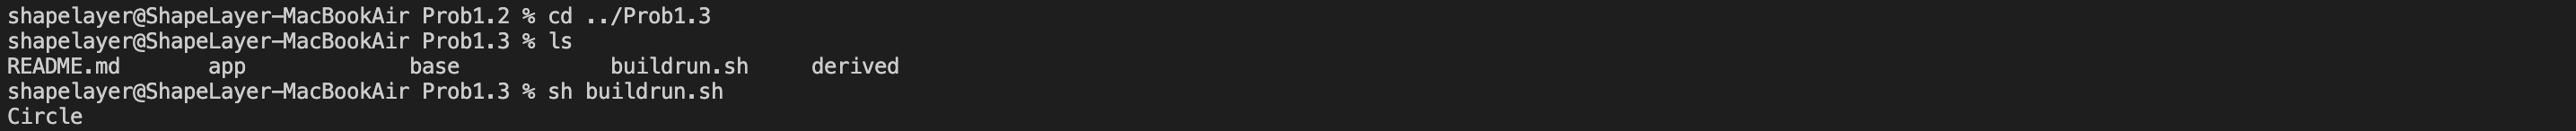
\includegraphics[width=\linewidth]{Prob1.3}
}



\section{과제2}
\subsection{소스 코드}
\javacode{java/Prob2/Prob2.java}
\subsection{실행 예제}
\makebox{
  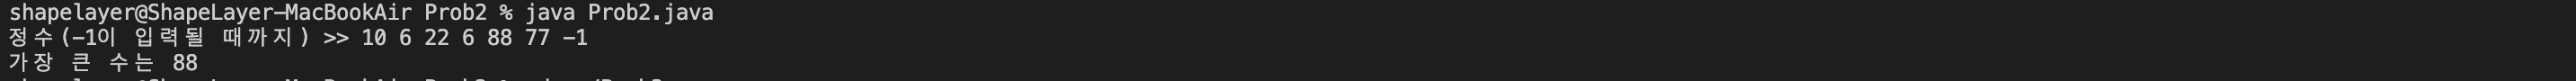
\includegraphics[width=\linewidth]{Prob2}
}


\section{과제3}
\subsection{소스 코드}
\javacode{java/Prob3/Prob3.java}
\subsection{실행 예제}
\makebox{
  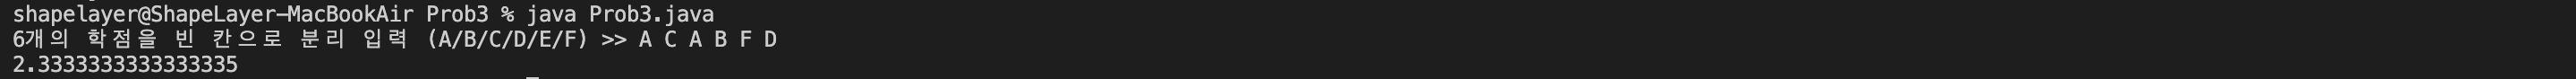
\includegraphics[width=\linewidth]{Prob3}
}


\end{document}
